% Options for packages loaded elsewhere
\PassOptionsToPackage{unicode}{hyperref}
\PassOptionsToPackage{hyphens}{url}
%
\documentclass[11pt]{article}
\usepackage{titlesec}

% \usepackage[numbers]{natbib} % ← removed (conflicts with biblatex)

\newcommand{\sectionbreak}{\clearpage}
\usepackage{amsmath,amssymb}
\usepackage{iftex}
\ifPDFTeX
  \usepackage[T1]{fontenc}
  \usepackage[utf8]{inputenc}
  \usepackage{textcomp} % provide euro and other symbols
\else % if luatex or xetex
  \usepackage{unicode-math} % this also loads fontspec
  \defaultfontfeatures{Scale=MatchLowercase}
  \defaultfontfeatures[\rmfamily]{Ligatures=TeX,Scale=1}
\fi
\usepackage{lmodern}
\ifPDFTeX\else
  % xetex/luatex font selection
\fi
% Use upquote if available, for straight quotes in verbatim environments
\IfFileExists{upquote.sty}{\usepackage{upquote}}{}
\IfFileExists{microtype.sty}{% use microtype if available
  \usepackage[]{microtype}
  \UseMicrotypeSet[protrusion]{basicmath} % disable protrusion for tt fonts
}{}
\makeatletter
\@ifundefined{KOMAClassName}{% if non-KOMA class
  \IfFileExists{parskip.sty}{%
    \usepackage{parskip}
  }{% else
    \setlength{\parindent}{0pt}
    \setlength{\parskip}{6pt plus 2pt minus 1pt}}
}{% if KOMA class
  \KOMAoptions{parskip=half}}
\makeatother
\usepackage{xcolor}
\usepackage{graphicx}
\makeatletter
\def\maxwidth{\ifdim\Gin@nat@width>\linewidth\linewidth\else\Gin@nat@width\fi}
\def\maxheight{\ifdim\Gin@nat@height>\textheight\textheight\else\Gin@nat@height\fi}
\makeatother
% Scale images if necessary, so that they will not overflow the page
% margins by default, and it is still possible to overwrite the defaults
% using explicit options in \includegraphics[width, height, ...]{}
\setkeys{Gin}{width=\maxwidth,height=\maxheight,keepaspectratio}
% Set default figure placement to htbp
\makeatletter
\def\fps@figure{htbp}
\makeatother
\ifLuaTeX
  \usepackage{luacolor}
  \usepackage[soul]{lua-ul}
\else
  \usepackage{soul}
\fi
\setlength{\emergencystretch}{3em} % prevent overfull lines
\providecommand{\tightlist}{%
  \setlength{\itemsep}{0pt}\setlength{\parskip}{0pt}}
\setcounter{secnumdepth}{-\maxdimen} % remove section numbering
\ifLuaTeX
  \usepackage{selnolig}  % disable illegal ligatures
\fi
\IfFileExists{bookmark.sty}{\usepackage{bookmark}}{\usepackage{hyperref}}
\IfFileExists{xurl.sty}{\usepackage{xurl}}{} % add URL line breaks if available
\urlstyle{same}
\hypersetup{
  pdftitle={Cellular Signal Coverage Mapping},
  hidelinks,
  pdfcreator={LaTeX via pandoc}}

\usepackage[style=numeric,sorting=none]{biblatex}
\addbibresource{references.bib}


\title{\LARGE \textbf{Cellular Signal Coverage Mapping}}
\author{\large Neta Cohen}
\date{\today}

\begin{document}

\maketitle

\hypertarget{abstract}{%
\section{1. Abstract}\label{abstract}}

This project presents a practical methodology for mapping and analyzing
cellular network coverage in underrepresented regions. Signal
measurements were collected across multiple locations and times, stored
in a cloud database, and processed with custom Python scripts to
generate detailed coverage maps. The maps reveal strong reception in
central Ariel but highlight significant gaps along rural roads,
illustrating the value of localized, empirical measurements. While
limited by the scale of data collection and reliance on a small number
of devices, the study demonstrates a replicable approach that can
support both researchers and local authorities in assessing and
improving mobile service quality.

{\small
\tableofcontents
}\newpage

\hypertarget{introduction}{%
\section{ 2. Introduction}\label{introduction}}

This chapter provides the background and rationale for the project,
explaining the gap in existing coverage data for underrepresented
regions and motivating the need for localized, empirical measurement
campaigns.

\hypertarget{background}{%
\subsection{2.1 Background}\label{background}}

Mobile network coverage has become a fundamental element of modern life,
enabling communication, access to essential services, and participation
in the digital economy. Reliable connectivity is no longer a luxury, but
a necessity. As mobile usage continues to grow, both users and service
providers increasingly depend on accurate coverage data to assess
service quality, identify connectivity issues, and plan infrastructure
deployment.

To meet this need, several platforms, most notably OpenSignal\cite{opensignal2024} and
CellMapper\cite{cellmapper2024}, offer crowdsourced coverage maps based on real-time signal
measurements contributed by users worldwide. These platforms provide
valuable insights and perform well in densely populated areas, where
large volumes of user contributions ensure frequent updates and high
spatial resolution. However, their effectiveness is uneven: in less
populated regions, where fewer users contribute data, coverage maps are
often incomplete, outdated, or misleading.

\hypertarget{motivation}{%
\subsection{2.2 Motivation}\label{motivation}}

In Israel, and particularly in semi-rural areas such as Ariel and the
Shomron (Samaria) region, substantial gaps persist in publicly available
coverage data. Weak or absent information makes it difficult for
residents, researchers, and policymakers to evaluate service quality or
plan infrastructure improvements.

This challenge is especially significant when considering emerging
technologies such as autonomous vehicles and unmanned aerial systems
(drones), which depend on continuous mobile connectivity for safe
navigation and real-time data transmission. Inconsistent or weak
coverage in rural regions can cause operational risks ranging from
navigation failures to loss of mission control.

The limitations of existing platforms are evident in their output.
Figure 1 shows OpenSignal's reported coverage for Ariel, which
significantly underrepresents actual network availability. Figure 2
contrasts OpenSignal's estimated antenna positions (left) with verified
locations from the official government dataset (right). The
discrepancies between estimated and verified infrastructure highlight
both the incompleteness of crowdsourced maps and the difficulties of
accessing accurate, user-friendly antenna data in Israel.

Together, these observations motivate the need for targeted, empirical
data collection to complement existing platforms. Accurate, localized
coverage maps are essential not only for improving consumer experience
but also for ensuring safety, accessibility, and infrastructure
readiness in regions underserved by global mapping tools.

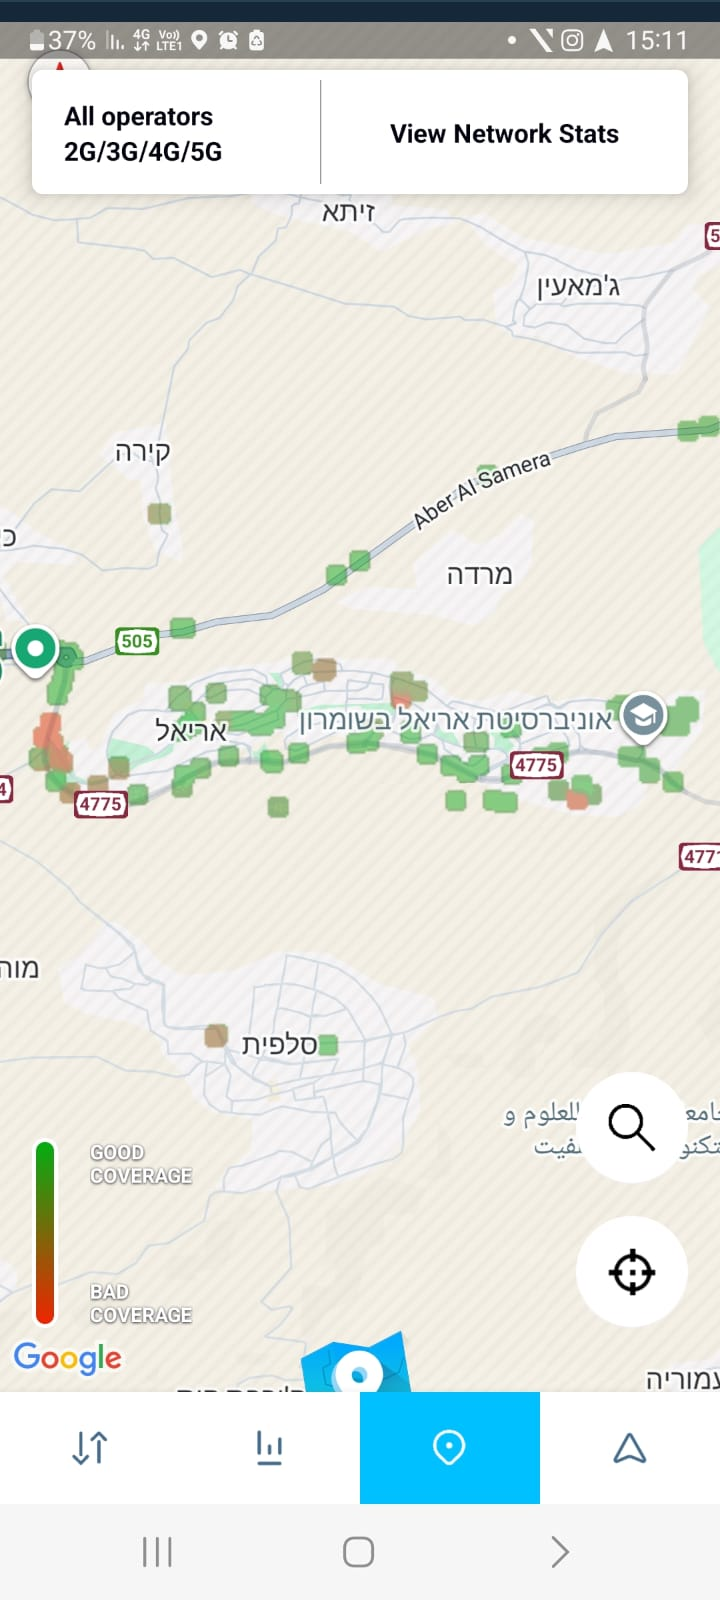
\includegraphics[width=1.56771in,height=3.49541in]{figures/media/image2.jpg}\\
\textbf{Figure 1.} Reported coverage for Ariel in OpenSignal, showing
sparse and incomplete representation of network availability.

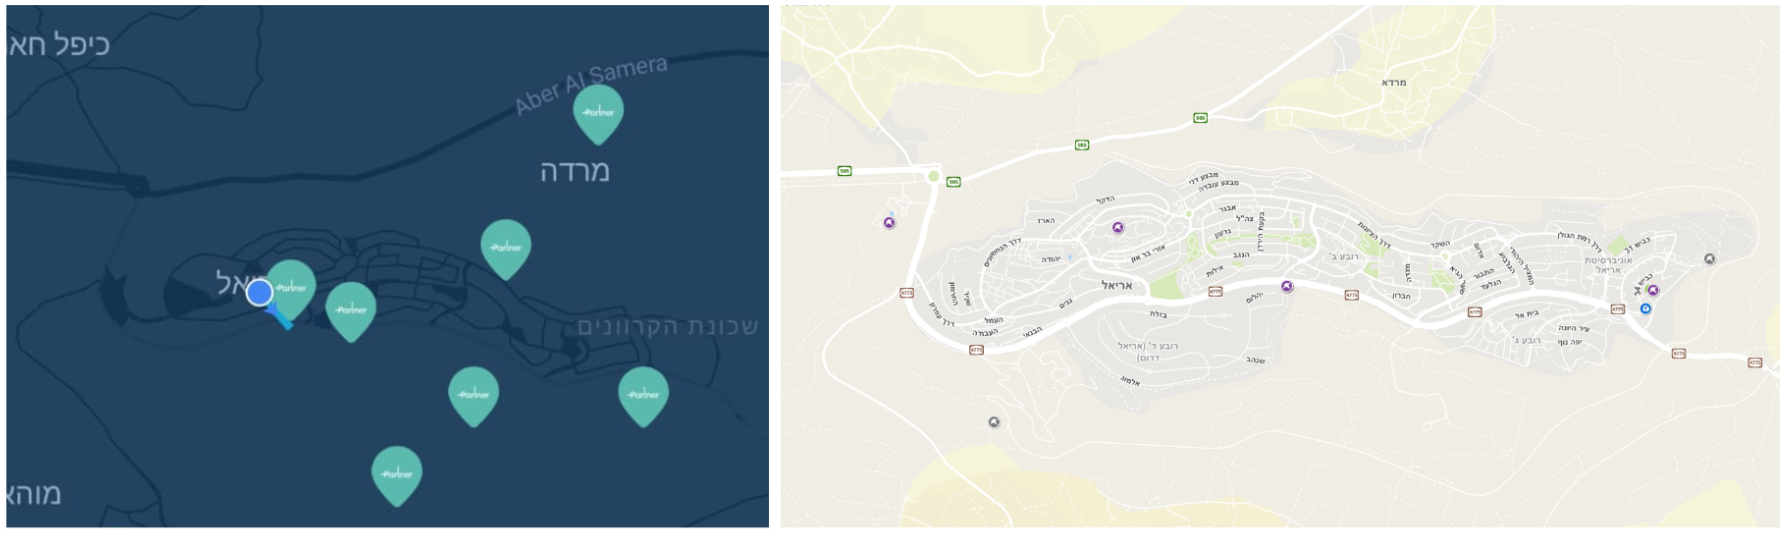
\includegraphics[width=1.0\textwidth]{figures/media/image1.png}
\textbf{Figure 2.} Antenna location data: OpenSignal's estimated
placements (left) versus verified locations from the official government
dataset (right).

\hypertarget{objectives}{%
\subsection{2.3 Objectives}\label{objectives}}

The primary objective of this project is to develop and apply a
replicable methodology for generating accurate mobile coverage maps in
underrepresented regions. Specifically, the project aims to:

\begin{itemize}
\item
  \begin{quote}
  Collect reliable signal measurements using mobile devices and the
  G-MoN Pro application.
  \end{quote}
\item
  \begin{quote}
  Store and organize these measurements in a structured cloud database
  (Firebase) for reproducibility and further analysis.
  \end{quote}
\item
  \begin{quote}
  Generate high-resolution coverage maps through Python-based processing
  and interpolation techniques that combine measurement data with
  antenna information.
  \end{quote}
\item
  \begin{quote}
  Demonstrate comparisons across dimensions such as time of day,
  geographic region, and coverage type.
  \end{quote}
\item
  \begin{quote}
  Provide open-source tools and documentation that enable others to
  replicate, extend, and apply the methodology in additional contexts.
  \end{quote}
\end{itemize}

It is hypothesized that systematic field measurements, even when limited
in scope, can yield coverage maps that are significantly more accurate
and representative than existing crowdsourced platforms in semi-rural
areas.

\hypertarget{related-challenge}{%
\subsection{2.4 Related Challenge: Positioning Without GPS}\label{related-challenge}}

Another challenge closely related to this study is the problem of inferring location without GPS. This topic has been extensively discussed in the literature \cite{youssef2005locating,bahl2000radar,kaplan2017}. 
While the present research focuses on estimating coverage quality based on known locations, the inverse problem aims to infer the user’s position from measured signal strengths. 
This task, often referred to as \emph{signal-based localization}, involves using radio measurements such as RSSI or RSRP to estimate geographic coordinates in the absence of satellite positioning data.

Although this study addresses the opposite direction, both problems share underlying signal-propagation characteristics and spatial modeling challenges. Understanding advances in signal-based localization may therefore help refine coverage estimation models and improve mapping accuracy.

\hypertarget{literature-review}{%
\section{3. Literature Review}\label{literature-review}}

This chapter reviews existing commercial platforms and academic research
in cellular coverage mapping. It highlights their contributions,
identifies common gaps and limitations, and clarifies how the current
project builds upon and extends previous work.

\hypertarget{market-solutions-for-network-coverage-mapping}{%
\subsection{3.1 Market Solutions for Network Coverage
Mapping}\label{market-solutions-for-network-coverage-mapping}}

Over the past decade, several commercial and open-source platforms have
emerged to measure and visualize mobile network coverage. These
solutions vary in methodology, ranging from crowdsourced user
contributions to structured drive-test campaigns.

OpenSignal is among the most widely used platforms worldwide. Its mobile
application collects parameters such as signal strength, data speed,
latency, and service availability, which are then aggregated into
interactive maps and benchmarking tools \cite{opensignal2024}. The strength
of OpenSignal lies in its continuously updated, large-scale dataset,
which makes it valuable for consumer-facing comparisons between
providers. However, the platform does not provide technical details such
as exact antenna locations or cell IDs, limiting its usefulness for
engineering-level analysis.

CellMapper takes a more infrastructure-oriented approach. While the
application runs, it records cell IDs, frequencies, GPS coordinates, and
signal strength, enabling users to map both tower locations and
associated coverage areas \cite{cellmapper2024}. This makes it particularly
valuable for engineers and researchers seeking insight into network
topology. Still, the platform depends heavily on active contributors,
and its maps often remain sparse or incomplete in less populated
regions. There is no coverage map in their site of Ariel and the
surrounding area.

Flycomm, an Israeli company, has developed an AI-powered solution for
monitoring and optimizing 3G, 4G, and 5G coverage \cite{flycomm2024}. It
combines crowdsourced data, dedicated drive tests, cloud-based
processing, and real-time visualization. The platform's strengths
include high accuracy, scalability, and full support for advanced mobile
standards, making it suitable for both operators and research purposes.
However, as a proprietary system, its methods and datasets are not fully
open to public validation, they provide service only for customers.

\hypertarget{academic-approaches-and-research}{%
\subsection{3.2 Academic Approaches and
Research}\label{academic-approaches-and-research}}

In parallel to commercial platforms, academic research has focused on
combining empirical measurements with geospatial and computational
analysis, aiming to achieve accurate and scalable coverage mapping.

Dharshini, Kumar, and Ramesh \cite{dharshini2022} proposed a low-cost
methodology that uses mobile devices to collect signal strength data
(RSSI), processed with open-source tools such as QGIS and Python. The
resulting geographic heatmaps highlight weak coverage areas while
remaining highly accessible for small-scale projects. However, data
collection still requires manual effort and is limited to local scopes.

More advanced frameworks leverage simulation and 3D modeling. The
Geo2SigMap system \cite{li2023} integrates OpenStreetMap data, Blender
models, and physical-layer simulation via Sionna to predict signal
strength using a cascaded U-Net architecture. Similarly, Choi et al.
\cite{choi2022} combined LiDAR-based 3D urban models with deep neural
networks to generate detailed propagation maps in dense environments.
Such models achieve strong predictive accuracy but rely heavily on
computational resources and structured geospatial inputs.

Recent work has also explored fusing multiple data sources and AI-based
approaches. Nguyen et al. \cite{nguyen2023} demonstrated multi-source
signal data fusion using crowdsensed and GPS inputs, improving
consistency in heterogeneous environments. Zhang et al. \cite{zhang2023}
and Ahmed and Kim \cite{ahmed2022} further advanced deep learning and
hybrid modeling techniques to estimate coverage from environmental and
propagation features, achieving reduced prediction errors compared to
classical models.

Finally, several studies have addressed the challenge of estimating
coverage in areas without direct measurements by incorporating antenna
locations and interpolation algorithms \cite{shepard1968}. While such
methods provide continuity between sampled points, their accuracy
depends strongly on data density and the availability of reliable
infrastructure metadata.

Despite the progress demonstrated by these studies, challenges remain in
translating advanced models and simulation-based methods into accessible,
field-validated solutions. The diversity of data sources, geographic
conditions, and modeling techniques highlights both the richness of the
research landscape and the ongoing need for practical, reproducible
approaches that can operate reliably in real-world environments.

\hypertarget{gaps-and-limitations-in-current-solutions}{%
\subsection{3.3 Gaps and Limitations in Current
Solutions}\label{gaps-and-limitations-in-current-solutions}}

While recent commercial and academic efforts have significantly advanced
coverage mapping, several challenges remain.

\begin{itemize}
\item
  \begin{quote}
  \textbf{Uneven data availability:} Crowdsourced measurements are
  concentrated in urban centers, leaving rural and peripheral regions
  with limited or outdated coverage information \cite{opensignal2024, cellmapper2024}.
  \end{quote}
\item
  \begin{quote}
  \textbf{Restricted technical details:} Many platforms limit access to
  essential identifiers such as cell IDs, frequencies, or antenna
  metadata, which are valuable for engineering-level analysis.
  \end{quote}
\item
  \begin{quote}
  \textbf{Resource-intensive field testing:} Dedicated drive-test
  campaigns provide accurate results but involve high costs and
  logistical effort \cite{flycomm2024}.
  \end{quote}
\item
  \begin{quote}
  \textbf{Model generalization and validation:} Machine-learning and
  hybrid models improve predictive accuracy \cite{li2023, zhang2023, ahmed2022}
  but often rely on simulated or localized datasets, limiting their
  transferability across environments.
  \end{quote}
\item
  \begin{quote}
  \textbf{Incomplete estimation of unmeasured areas:} Most systems show
  only direct measurements without extending coverage to unmeasured
  zones. Interpolation techniques exist \cite{shepard1968} but are rarely
  integrated into public or open-access mapping tools.
  \end{quote}
\end{itemize}

These factors highlight the ongoing need for practical, transparent, and
reproducible methods that bridge empirical data collection with scalable
prediction, particularly in regions that lack consistent measurement
coverage.


\hypertarget{relevance-to-the-current-project}{%
\subsection{3.4 Relevance to the Current
Project}\label{relevance-to-the-current-project}}

The present project directly addresses several of the remaining
challenges in current coverage mapping research. By collecting
real-world measurements in underrepresented areas, it produces detailed
and up-to-date maps that reflect actual on-ground conditions. The
workflow integrates targeted field data collection with automated
processing and visualization, providing results that are useful for both
local users and technical stakeholders.

While inspired by the open-source and low-cost approach of Dharshini et
al. \cite{dharshini2022}, this project enhances accessibility by
streamlining both data collection and visualization through Python
scripts and a structured Firebase backend. Similarly, while drawing from
the integration of field data and modeling in Geo2SigMap
\cite{li2023}, it prioritizes practical deployment and transparency over
computational complexity.

Recent studies have introduced advanced AI-based prediction methods
\cite{zhang2023, ahmed2022}, yet most rely on simulated datasets rather
than extensive real-world campaigns. In contrast, this project emphasizes
empirical validation, combining raw measurements with antenna metadata
and interpolation techniques \cite{shepard1968} to estimate coverage in
unmeasured areas. This produces continuous and realistic coverage maps,
particularly valuable in regions with sparse measurement density.

Finally, the project contributes to reproducibility by releasing
open-source code and a transparent methodology, enabling other
researchers and practitioners to replicate or adapt the workflow for
different locations and network conditions.


\hypertarget{system-overview-methodology}{%
\section{4. System Overview /
Methodology}\label{system-overview-methodology}}

This chapter outlines the methodology, architecture, and tools used to
design and implement the cellular coverage mapping system. Beyond
documenting the technical process, an important aim of this work is
knowledge sharing: by publishing the workflow and open-source code on
GitHub, the project provides a practical blueprint that others can
replicate, adapt to their own regions, or extend with new features.

\hypertarget{general-approach}{%
\subsection{4.1 General Approach}\label{general-approach}}

The project set out to map and analyze the quality of mobile network
service in the target region. To achieve this, field measurements were
conducted with the G-MoN Pro application \cite{gmon2023}, which
captures real-time cellular and GPS parameters during drive tests. These
measurements were processed, cleaned, and stored in a dedicated cloud
backend, creating a structured and continuously updatable database. This
database then served as the foundation for generating interactive
coverage maps using inverse distance weighting (IDW) interpolation
\cite{shepard1968}, and for conducting network performance analysis.

\hypertarget{tools-and-technologies}{%
\subsection{4.2 Tools and Technologies}\label{tools-and-technologies}}

The project integrates a set of tools that together form the pipeline
for data collection, storage, processing, and visualization. Each tool
fulfills a distinct role, ensuring that the system is both accurate and
scalable, while producing outputs that are meaningful for technical
analysis and accessible for broader stakeholders.

\hypertarget{g-mon-pro-data-collection}{%
\subsubsection{4.2.1 G-MoN Pro (Data
Collection)}\label{g-mon-pro-data-collection}}

The G-MoN Pro mobile application\cite{gmon2023} was the primary tool for collecting raw
cellular and GPS data during drive tests (see Figure 3). It records a wide range of
parameters in real time, including:

\begin{itemize}
\item
  \begin{quote}
  \textbf{Network identification:} PLMN, network type (2G/3G/4G/5G),
  cell IDs, frequency bands.
  \end{quote}
\item
  \begin{quote}
  \textbf{Signal strength and quality:} RSSI, RSRP, RSRQ, SNR, CQI.
  \end{quote}
\item
  \begin{quote}
  \textbf{Geolocation:} GPS coordinates, speed, accuracy, Timing
  Advance.
  \end{quote}
\item
  \begin{quote}
  \textbf{Throughput and capacity:} Uplink/downlink throughput,
  bandwidth, carrier aggregation.
  \end{quote}
\item
  \begin{quote}
  \textbf{5G-specific metrics:} NR state, synchronization signal
  strength, SINR, channel state information.
  \end{quote}
\item
  \begin{quote}
  \textbf{Metadata:} Timestamps, roaming status, database lookup
  references.
  \end{quote}
\end{itemize}

These measurements enabled both quantitative analysis of network
performance and visualization of coverage gaps, handover behavior, and
operator differences.
Notably, G-MoN Pro is capable of recording many of these radio and location parameters even without an active SIM card, as the device modem can still detect and log broadcasted cellular signals from nearby base stations.

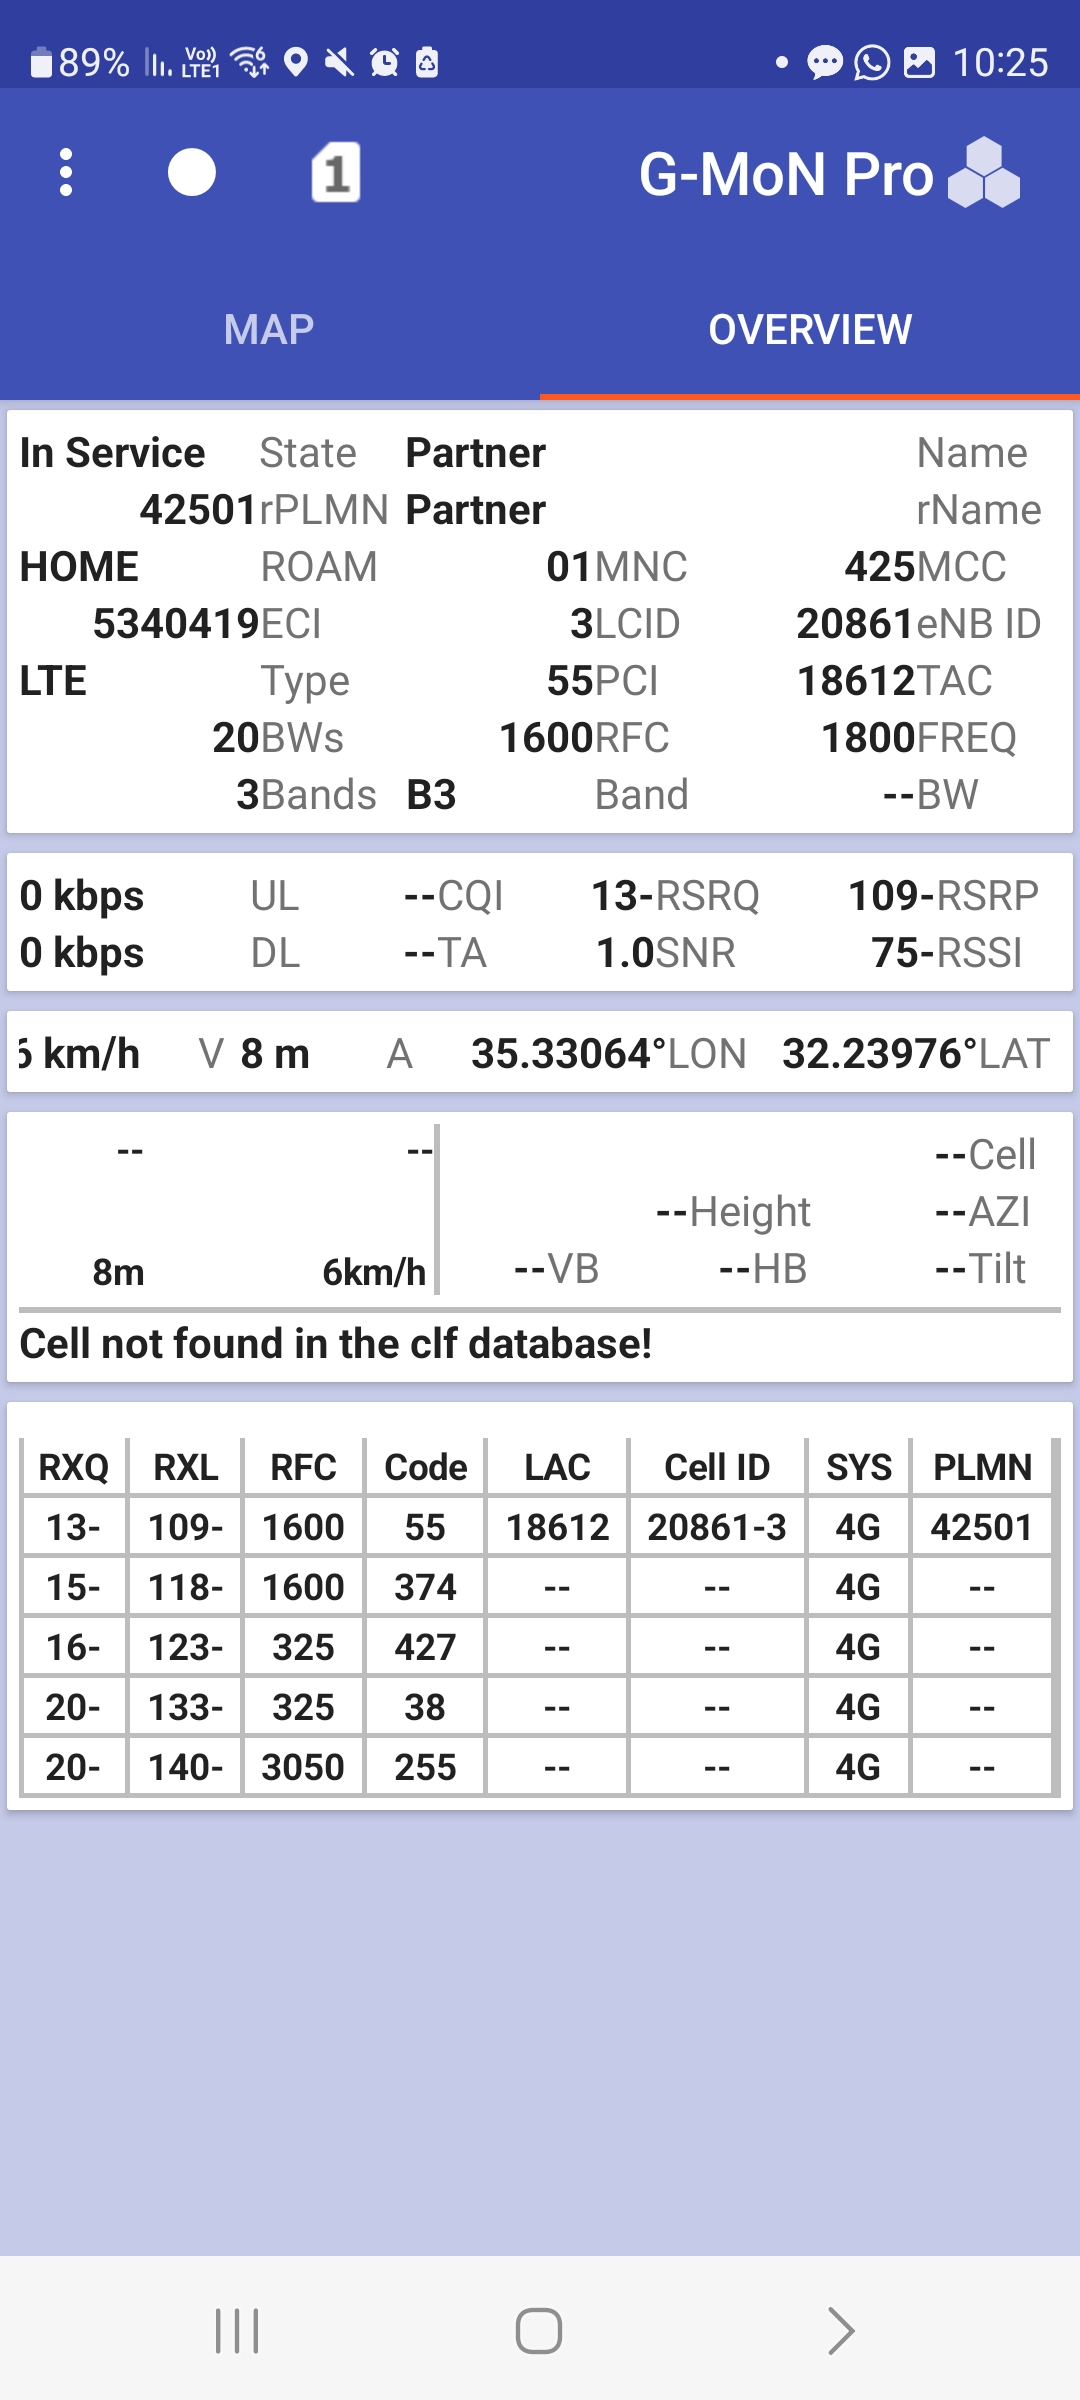
\includegraphics[width=1.56771in,height=3.49541in]{figures/media/gmonImage.png}\\
\textbf{Figure 3.} G-Mon Pro application data collection screen.

\hypertarget{firebase-database-and-cloud-backend}{%
\subsubsection{4.2.2 Firebase (Database and Cloud
Backend)}\label{firebase-database-and-cloud-backend}}

The system uses Firebase\cite{firebase2025} as its cloud-based backend, providing scalable
data storage, real-time synchronization, and secure user management.
Firebase served as the central repository where raw and processed data
were stored and organized. The database was structured into four key
collections:

\begin{enumerate}
\def\labelenumi{\arabic{enumi}.}
\item
  \begin{quote}
  \emph{Users}\\
  User profiles and associated provider information, enabling secure
  access and filtering of contributions.
  \end{quote}
\item
  \begin{quote}
  \emph{Data}\\
  As shown in Figure 4, each measurement in the Firebase \emph{Data}
  collection is stored as a structured document, identified by a unique
  \emph{user\_date\_time} key and containing both signal parameters and
  GPS metadata.
  \end{quote}
\item
  \begin{quote}
  \emph{BaseStations}\\
  A reference collection of known cell towers (ID, coordinates,
  provider, frequency bands), allowing validation and comparison with
  measured data.
  \end{quote}
\item
  \begin{quote}
  \emph{Maps}\\
  Processed coverage maps, organized by region, operator, and time
  period.
  \end{quote}
\end{enumerate}

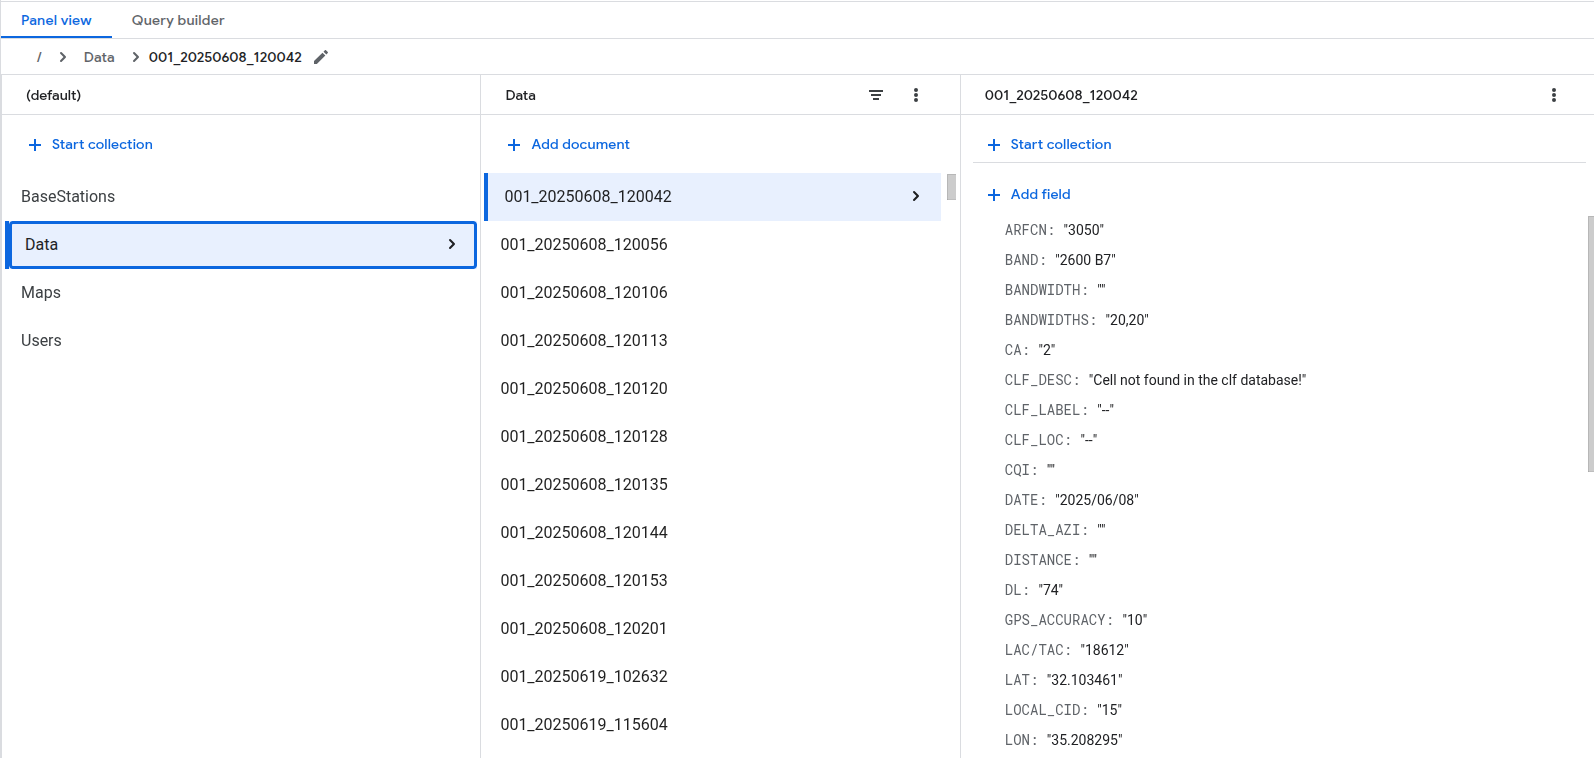
\includegraphics[width=1.0\textwidth]{figures/media/image7.png}\\
\textbf{Figure 4.} \emph{Data} collection in the Firebase database. Each
document represents a single measurement, indexed by a unique key
(\emph{user\_date\_time}) and containing signal parameters together with
GPS coordinates.

\hypertarget{python-data-processing-and-analysis}{%
\subsubsection{4.2.3 Python (Data Processing and
Analysis)}\label{python-data-processing-and-analysis}}

Python\cite{python2025} served as the main programming environment for this project,
supporting both data handling and coverage map generation. Since raw
G-MoN Pro logs often contained unstructured or duplicate entries, Python
scripts were essential for cleaning, preprocessing, and ensuring the
consistency of the dataset.

Key processing tasks included:

\begin{itemize}
\item
  \begin{quote}
  Parsing raw measurement logs into structured datasets.
  \end{quote}
\item
  \begin{quote}
  Extracting relevant rows from the Firebase database before generating
  specific coverage maps.
  \end{quote}
\item
  \begin{quote}
  Linking signal measurements with antenna location data to support
  spatial analysis.
  \end{quote}
\item
  \begin{quote}
  Generating KML layers for visualization in Google Earth.
  \end{quote}
\end{itemize}

In addition to preprocessing, Python was central to the creation of the
coverage maps themselves. The code implemented an interpolation approach
based on inverse distance weighting (IDW), a method that assigns greater
influence to nearby measurements\cite{shepard1968}. This technique made it
possible to estimate signal strength in unmeasured areas, producing
smooth, realistic coverage surfaces that combined raw field data with
antenna locations.

Python was also used to automate data management tasks, including
uploading new measurement files to Firebase, downloading filtered
subsets for map generation, and exporting finalized maps back into the
database for storage and retrieval.

The flexibility of Python enabled rapid iteration, testing of multiple
visualization styles, and reliable integration of the measurement,
storage, and mapping components. This ensured that outputs were
accurate, reproducible, and well aligned with the project's analytical
goals.

\hypertarget{google-earth-kml-visualization}{%
\subsubsection{4.2.4 Google Earth / KML
(Visualization)}\label{google-earth-kml-visualization}}

For visualization, processed datasets were converted into KML files and
displayed in Google Earth\cite{googleearth2025}. This stage transformed abstract measurements
into intuitive geographic insights. Signal quality represented by
gradient lines or shaded areas, with clear distinction between strong
and weak coverage zones.

Through this visualization layer, raw cellular data was turned into
actionable insights, allowing both technical specialists and
decision-makers to understand and evaluate coverage in the studied
region.

\hypertarget{workflow-diagram}{%
\subsection{4.3 Workflow Diagram}\label{workflow-diagram}}

The workflow of the system is illustrated in Figure 5. Data collection
begins with GMon Pro, which records cellular measurements during a drive
and exports them as a CSV file. The raw data is then uploaded to the
Firebase database using a Python script, ensuring that it is stored
securely and can be accessed for later processing. To generate maps,
data is retrieved from the database according to selected parameters
such as geographic area or time range. Using additional Python scripts,
the relevant data is exported back into CSV format. Then the data is
processed into a KML file, which can be visualized in Google Earth. The
mapping scripts allow for flexible outputs, such as maps with or without
cell tower locations, maps showing only sampled points, or broader
coverage visualizations distinguishing between internet and call
services. Finally, the generated maps are displayed in Google Earth for
analysis and also stored back in the database for archiving and further
use. In this way, the workflow connects raw field measurements with
meaningful geographic visualizations, creating a complete and
reproducible pipeline for cellular coverage mapping.

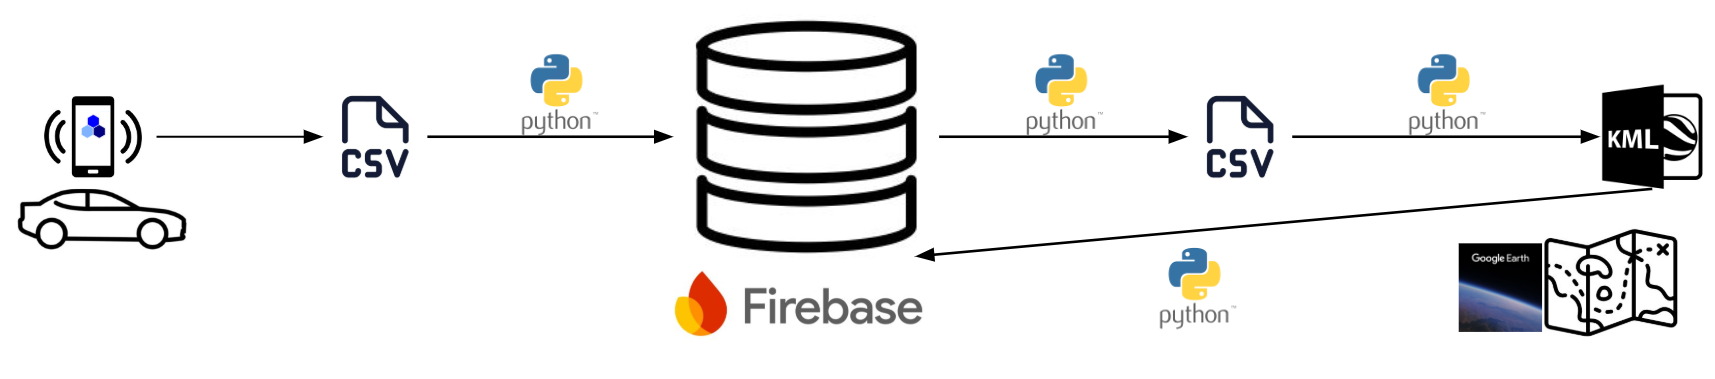
\includegraphics[width=1.0\textwidth]{figures/media/image3.png}\\
\textbf{Figure 5.} Workflow of the cellular coverage mapping system,
from data collection with GMon Pro to storage in Firebase, processing
with Python, and visualization in Google Earth.

\hypertarget{challenges-in-data-collection}{%
\subsection{4.4 Challenges in Data
Collection}\label{challenges-in-data-collection}}

A major challenge in this project was obtaining reliable information on
antenna locations and identifiers. Since no publicly accessible database
provides complete and up-to-date details, this information had to be
derived manually. The process required cross-referencing field
measurements with available infrastructure data to identify cell towers
and their corresponding identifiers. Complicating matters further, a
single antenna can appear under multiple identifiers depending on
factors such as reception angle and frequency band.

Although time-consuming, this effort greatly enhanced the value of the
project by producing an organized and up-to-date dataset of antennas and
signal measurements in the region. Beyond serving as the foundation for
the present analysis, such a dataset can support future research, assist
local councils in infrastructure planning, and potentially be integrated
into national databases, ultimately improving the accessibility,
accuracy, and efficiency of coverage information for the wider public.

\hypertarget{color-representation-in-coverage-maps}{%
\subsection{4.5 Color Representation in Coverage Maps}\label{color-representation-in-coverage-maps}}

Before moving on to the results section, it is important to clarify the meaning of the colors used in the coverage maps.

The color scale reflects the signal strength values measured or predicted at each location. Colors range from red, indicating weak signal, through yellow for moderate reception, to green for strong signal.

Technically, the values correspond to the received signal power (RSRP for LTE or RSCP/RSSI for other technologies), expressed in decibel-milliwatts (dBm). Higher (less negative) values such as –60 dBm indicate excellent reception and high data throughput potential, whereas lower values below –110 dBm represent poor or unreliable connectivity. 

In the maps, green shades represent strong signals above –80 dBm, yellow tones correspond to moderate reception between –80 dBm and –100 dBm, and red shades indicate weak signals below –100 dBm.
This color-based representation allows the map to visually communicate variations in network performance across the city, making it easy to identify both strong coverage areas and locations where service quality may degrade.


\hypertarget{results-and-analysis}{%
\section{5. Results and Analysis}\label{results-and-analysis}}

This chapter reports the results of the coverage mapping and provides
analysis of key findings.

\hypertarget{coverage-maps-of-ariel}{%
\subsection{5.1 Coverage Maps of Ariel}\label{coverage-maps-of-ariel}}

The central outcome of this study is a detailed cellular coverage map of
the city of Ariel, visualized through a color-coded representation of
signal quality. The map highlights the locations of base stations as
well as surrounding areas of strong and weak reception. Overall,
coverage across most of the city is satisfactory, with several base
stations providing overlapping service.

To ensure reliability, the dataset was filtered by provider, geographic
boundaries, and measurement period, so that the map reflects the
performance of a single operator under consistent conditions. After
filtering, 5,391 measurements remained and were used to generate the
coverage surface shown in Figure 6. The surface was created using
inverse distance weighting (IDW) interpolation, which combines actual
measurement points with known antenna locations. In this process,
measurements closer to a given point have stronger influence, while
antenna proximity is used to refine predictions. As a result, unmeasured
areas are estimated realistically, with accuracy improving as
measurement density increases.

This approach produces a high-resolution visualization that reveals both
expected and less obvious patterns. In central Ariel, where data points
are dense and multiple antennas overlap, the map shows stable and
redundant coverage. At the city's edges, however, coverage rapidly
shifts from strong to weak, often corresponding to line-of-sight
obstructions or distance from the nearest tower. Importantly, the method
also identifies ``shadow zones'' behind buildings or in complex terrain,
which would be difficult to detect from measurements alone.

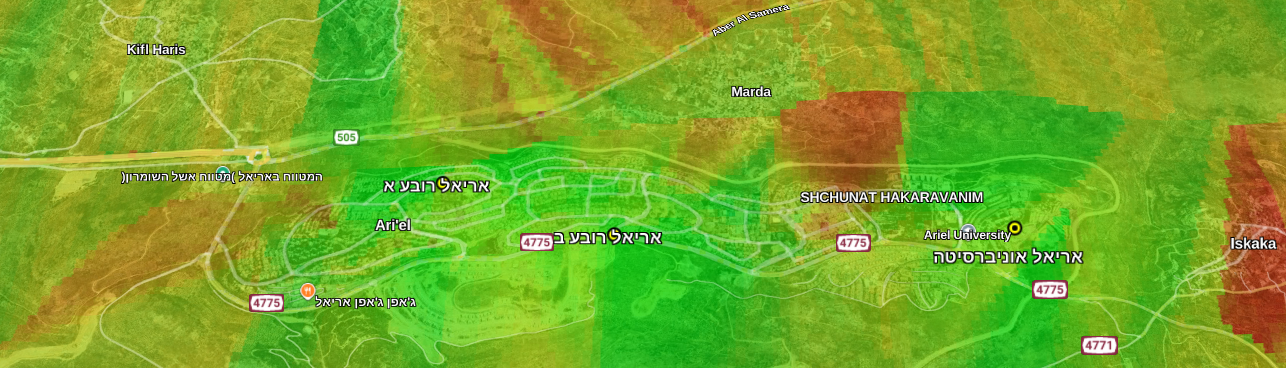
\includegraphics[width=1.0\textwidth]{figures/media/image6.png}\\
\textbf{Figure 6.} Predicted cellular coverage in Ariel for provider
PHI, based on 5,391 filtered measurement points.

\hypertarget{comparing-reception-between-times-of-day}{%
\subsection{5.2 Comparing reception between times of
day}\label{comparing-reception-between-times-of-day}}

Cellular reception in Ariel shows subtle variation between daytime and
nighttime conditions. Figure 7 presents the coverage map generated from
measurements collected between 07:00 and 21:00, while Figure 8
illustrates the corresponding map based on nighttime measurements
(21:00--07:00). During the day, coverage remains generally strong, but
more yellow and orange patches are visible, particularly at the city's
periphery. At night, coverage appears slightly better, with broader and
more continuous green areas indicating stable reception.

These differences suggest that time-of-day effects can influence
perceived coverage quality. One possible explanation is reduced network
load at night, which lowers interference and improves reception.
Environmental conditions such as temperature inversions may also affect
radio propagation, while the distribution of measurement routes may play
a secondary role.

Daytime coverage was modeled using 4,207 measurements (Figure 7), while
the nighttime map (Figure 8) is based on 1,925 measurements. Although
the smaller nighttime dataset may lead to a somewhat coarser
interpolation, the overall trends remain consistent. Both maps confirm
that reception in Ariel is generally strong, with only modest variation
between time periods.

Although the observed differences are relatively modest, this comparison
illustrates the flexibility of the mapping framework. The same approach
can be extended to a variety of scenarios: comparing different service
providers, analyzing coverage across multiple years, or contrasting
internet (data) performance with voice call connectivity. By filtering
the Firebase database for the relevant subset of measurements, maps can
be generated and compared under consistent conditions. This demonstrates
that the project is not limited to producing a single coverage snapshot,
but rather offers a scalable tool for systematic comparison across
dimensions of time, operator, and service type.

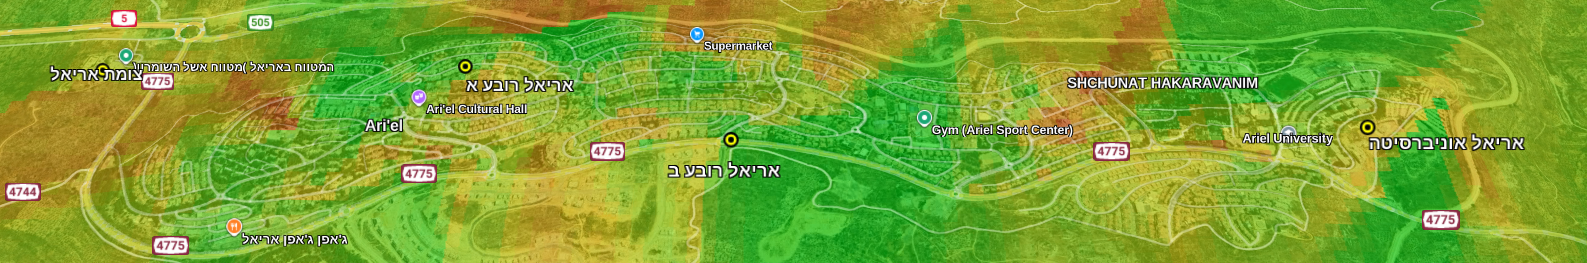
\includegraphics[width=1.0\textwidth]{figures/media/image9.png}\\
\textbf{Figure 7.} Predicted cellular coverage in Ariel during daytime
hours (07:00--21:00), based on 4,207 filtered measurements. Coverage is
generally strong, though more yellow and orange patches appear at the
city's periphery.

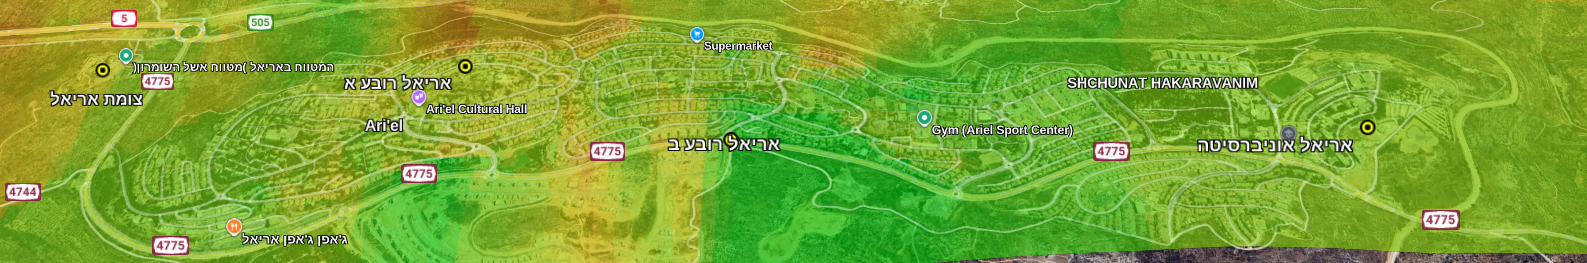
\includegraphics[width=1.0\textwidth]{figures/media/image5.png}\\
\textbf{Figure 8.} Predicted cellular coverage in Ariel during nighttime
hours (21:00--07:00), based on 1,925 filtered measurements. Coverage
appears slightly stronger, with broader green areas indicating more
stable reception.

\hypertarget{road-segment-coverage}{%
\subsection{5.3 Road Segment Coverage}\label{road-segment-coverage}}

The coverage map along the road from Ariel to Elon Moreh demonstrates
clear fluctuations in cellular service quality. As shown in Figure 9,
certain segments maintain stable reception (indicated in green and
yellow) with strong RSRP and SNR values, whereas other areas,
particularly near sharp curves, valleys, and elevated terrain, exhibit
rapid signal degradation (orange to red, and in some places blue). These
fluctuations often result from topographic obstacles that block
line-of-sight to the serving cell, forcing the device to switch to a
weaker sector or a more distant antenna. In sections such as Figure 10,
frequent handovers between neighboring cells are visible, marked by
sudden changes in cell identifiers along the route, and reflected in
abrupt shifts in color. A more prolonged weak-coverage area is
highlighted in Figure 11, where topographic barriers consistently
restrict signal strength for extended distances. While the figures are
based on a single provider, additional measurements indicate that other
networks display similar patterns in these areas, suggesting that the
primary cause lies in the terrain rather than in provider-specific
infrastructure.

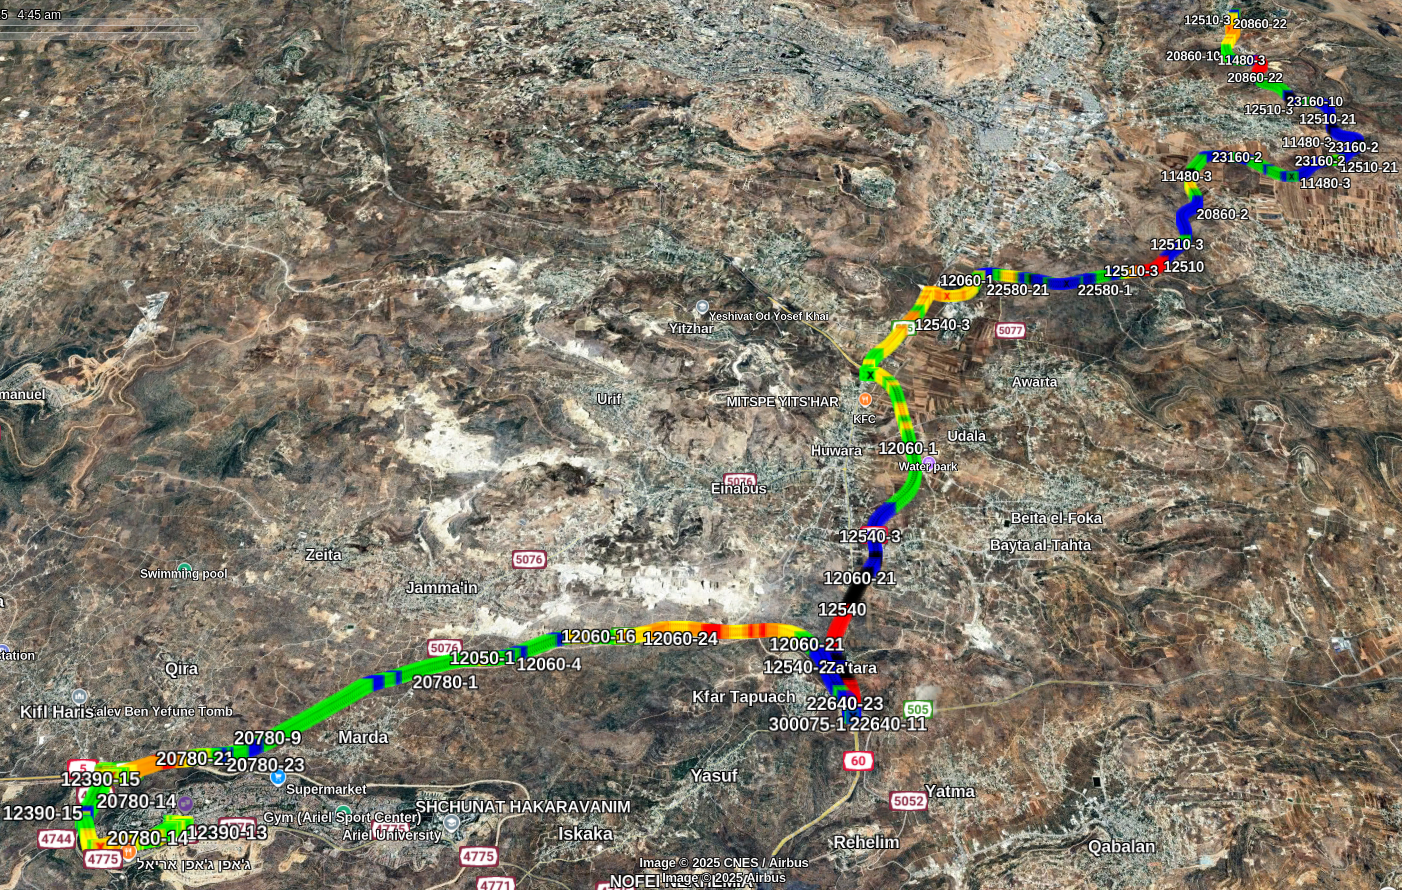
\includegraphics[width=3.56458in,height=2.24773in]{figures/media/image11.png}\\
\textbf{Figure 9.} KML output from G-Mon Pro, illustrating alternating
strong and weak coverage along a winding road segment, reflecting
topographic influence.

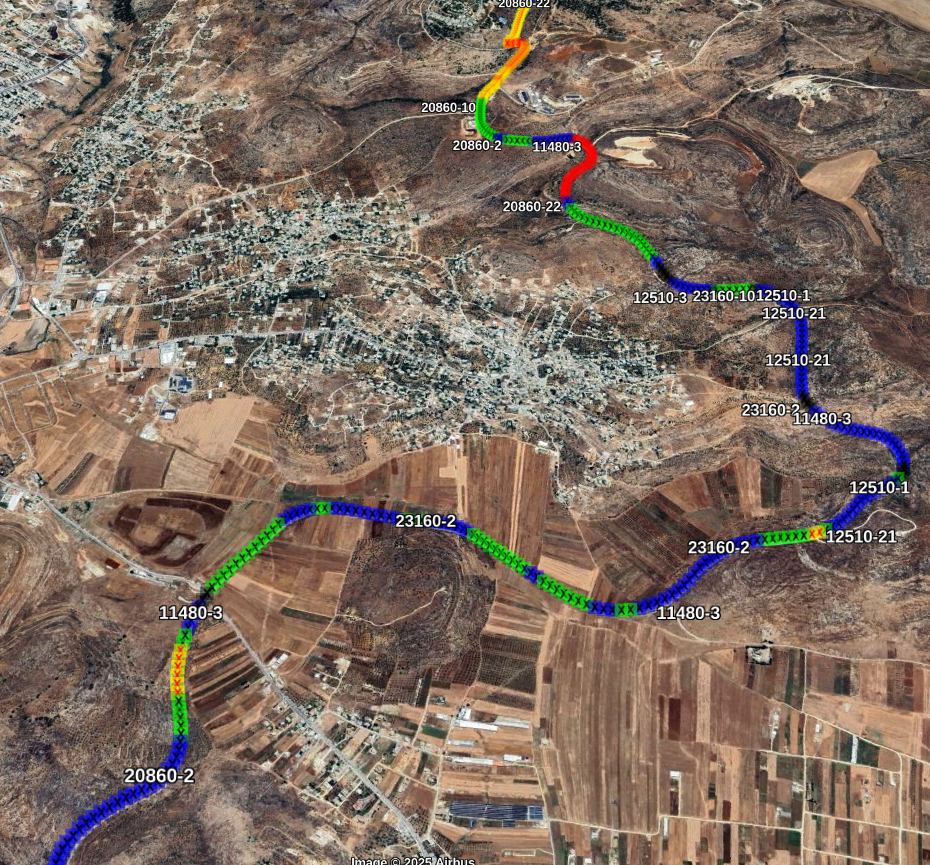
\includegraphics[width=2.98125in,height=2.7956in]{figures/media/image10.png}\\
\textbf{Figure 10.} KML output from G-Mon Pro, showing frequent handovers
between neighboring cells and rapid changes in signal quality.\\
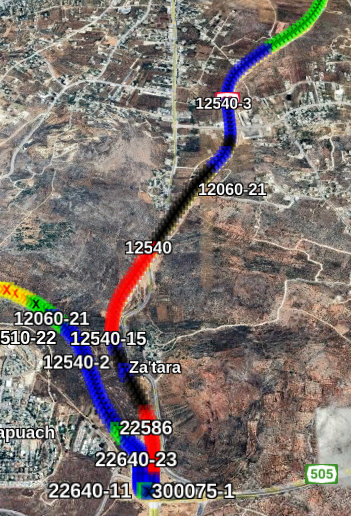
\includegraphics[width=1.87708in,height=2.78502in]{figures/media/image4.png}\\
\textbf{Figure 11.} KML output from G-Mon Pro, highlighting persistent
low coverage in a valley region, observed consistently across multiple
providers.

\hypertarget{contribution-of-the-study}{%
\subsection{5.4 Contribution of the
Study}\label{contribution-of-the-study}}

This study makes several contributions to both practice and research:

\begin{itemize}
\item
  \begin{quote}
  \textbf{High-resolution coverage maps:} Produced detailed maps of the
  city of Ariel and surrounding roads, offering a resource for local
  authorities, service providers, and the public.
  \end{quote}
\item
  \begin{quote}
  \textbf{Replicable methodology:} Introduced a simple, adaptable
  workflow that can be applied in other regions and extended for future
  studies.
  \end{quote}
\item
  \begin{quote}
  \textbf{Open-source tools:} Released code that enables researchers and
  practitioners to extend the analysis, refine algorithms, and generate
  new comparisons.
  \end{quote}
\item
  \begin{quote}
  \textbf{Comparative potential:} Demonstrated that coverage maps can be
  compared across multiple dimensions---such as times of day, providers,
  years, or service types (data vs. voice)---to identify trends and
  contextualize service quality.
  \end{quote}
\item
  \begin{quote}
  \textbf{Updated antenna dataset (technical note):} Compiled an updated
  set of antenna locations in the region, which, while not the main
  focus, adds value by improving map accuracy and supporting future
  analysis.
  \end{quote}
\end{itemize}

The findings highlight two main conclusions:

\begin{itemize}
\item
  \begin{quote}
  \textbf{Urban coverage:} Within Ariel, reception is generally
  sufficient, supported by overlapping antennas, though small pockets of
  weak service remain.
  \end{quote}
\item
  \begin{quote}
  \textbf{Rural gaps:} Along the road to Elon Moreh, large stretches of
  weak or absent connectivity persist, with potential consequences for
  accessibility and safety.
  \end{quote}
\end{itemize}

Overall, this analysis demonstrates the value of combining raw field
measurements with geographic knowledge and interpolation techniques. The
resulting maps provide a fine-grained, realistic picture of mobile
coverage, while also illustrating the potential of community-driven,
empirical data collection to complement and refine official coverage
maps.


\hypertarget{limitations}{%
\section{6. Limitations}\label{limitations}}

This chapter discusses the limitations of the study and their
implications for the validity and generalizability of the results.

\hypertarget{limited-data}{%
\subsection{6.1 Limited Data}\label{limited-data}}

Most measurements in this study were collected from a single provider
(PHI), limiting the ability to compare operators systematically. While
coverage patterns appeared broadly similar across other networks, a
comprehensive multi-provider analysis was not possible. In addition,
fewer measurements were available for nighttime hours, resulting in
lower resolution for those maps. This imbalance may slightly influence
the observed patterns, and future work should aim to collect more evenly
distributed data across providers and time periods.

\hypertarget{accuracy-and-dependence-on-data-density}{%
\subsection{6.2 Accuracy and Dependence on Data
Density}\label{accuracy-and-dependence-on-data-density}}

The accuracy of the generated maps depends heavily on measurement
density. In central Ariel, where many points were collected, the maps
closely reflect real-world conditions. In sparsely measured areas,
however, the interpolation may underestimate coverage or exaggerate weak
zones, as illustrated in Figure 12. Expanding data collection through
additional fieldwork or crowdsourcing would improve the reliability of
future maps.

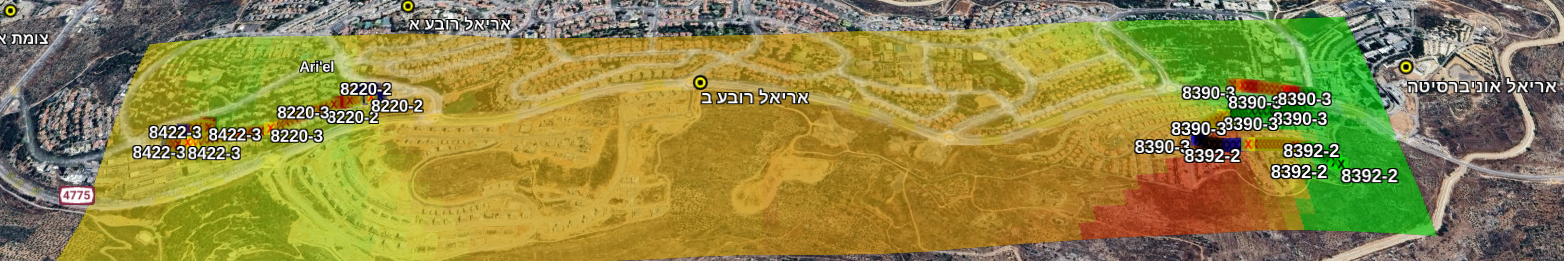
\includegraphics[width=1.0\textwidth]{figures/media/image8.png}\\
\textbf{Figure 12.} Example of a coverage map generated from a sparse
dataset. With too few measurement points, interpolation produces broad
and less reliable zones of weak reception, which may not fully reflect
real user experience.

\hypertarget{methodological-assumptions}{%
\subsection{6.3 Methodological
Assumptions}\label{methodological-assumptions}}

The interpolation method (IDW) assumes that coverage changes smoothly
with distance. While effective for producing a continuous map, this
approach cannot fully capture sudden drops in reception caused by
terrain, buildings, or network management. The maps should therefore be
viewed as realistic approximations rather than exact reflections of user
experience.

As a technical note, all data was collected on Android devices using the
G-MoN Pro app; differences in hardware or software could introduce minor
measurement bias. Additionally, the study focused on signal strength
rather than user-facing metrics such as throughput or call quality.


\hypertarget{discussion-and-implications}{%
\section{7. Discussion and
Implications}\label{discussion-and-implications}}

This chapter discusses the practical value of the findings and outlines
directions for future research.

\hypertarget{usefulness-for-municipalities-and-researchers}{%
\subsection{7.1 Usefulness for Municipalities and
Researchers}\label{usefulness-for-municipalities-and-researchers}}

The maps and methodology developed in this study have direct practical
value for both municipalities and researchers. For local authorities,
high-resolution coverage maps provide actionable insights into areas of
weak reception that may affect accessibility, safety, and urban
development planning. Municipal decision-makers can use such information
when engaging with service providers or considering infrastructure
investments, ensuring that underserved areas receive attention.

For researchers, the study demonstrates how empirical signal
measurements, combined with interpolation techniques and open-source
tools, can generate reliable and fine-grained coverage maps. The
replicable framework allows future studies to extend the analysis to
additional regions, test alternative interpolation methods, or integrate
supplementary datasets. The implemented system is readily adaptable for
importing measurement data from other regions, enabling the generation
of diverse coverage maps with minimal configuration. This positions the
project as a bridge between technical research and applied urban policy.


\hypertarget{future-research-directions}{%
\subsection{7.2 Future Research
Directions}\label{future-research-directions}}

There are several ways to improve and expand this work:

\begin{itemize}
\item
  \begin{quote}
  \textbf{Expanding geographic scope:} Extending data collection across
  additional regions of Israel and abroad, particularly rural and semi-urban areas,
  would provide a more representative national picture of mobile
  connectivity.
  \end{quote}
\item
  \begin{quote}
  \textbf{Crowdsourcing at scale:} Encouraging contributions from a
  larger pool of users could improve spatial and temporal coverage,
  while reducing route-specific bias. This aligns with the broader
  concept of participatory sensing, in which communities collectively
  contribute data to generate shared knowledge \cite{burke2006}.
  \end{quote}
\item
  \begin{quote}
  \textbf{Automated analytics:} Incorporating advanced methods such as
  machine learning could enable the detection of anomalies, prediction
  of coverage quality, and modeling of future infrastructure needs.
  \end{quote}
\item
  \begin{quote}
  \textbf{User-facing tools:} Developing a web-based or mobile interface
  would make it possible for end users to view and compare real-time
  coverage maps for their location and provider, fostering transparency
  and empowering consumers.
  \end{quote}
\item
  \begin{quote}
  \textbf{Localization research:} The collected signal data could also
  support studies on estimating device location from cellular
  measurements, contributing to the development of positioning methods
  that operate without GPS \cite{youssef2005locating,bahl2000radar,kaplan2017}.
  \end{quote}

\end{itemize}

By combining these extensions, the system can evolve from a research
prototype into a comprehensive, open, and continuously updated platform
for evaluating mobile service quality in Israel and beyond.

\hypertarget{conclusion}{%
\section{8. Conclusion}\label{conclusion}}

This project demonstrates a practical and replicable methodology for
mapping and analyzing mobile network coverage in underrepresented
regions. Using G-MoN Pro for real-time signal measurement, Firebase for
centralized data management, and automated visualization scripts, it was
possible to generate detailed coverage maps of Ariel and the surrounding
area. The results revealed both areas of strong, overlapping coverage
and critical connectivity gaps, offering actionable insights for users,
researchers, municipalities, and service providers.

Except for generating coverage maps, the study also contributed an
open-source workflow that others can adapt and extend, as well as an
updated antenna dataset that improves accuracy for future analyses. It
further demonstrated how comparative analyses across providers, times,
and service types can reveal patterns and contextualize service quality.
These contributions highlight the broader research and practical value
of empirical, community-driven data collection in refining and
complementing official coverage maps.

Overall, the project illustrates the value of combining community-driven
data collection with geographic modeling techniques to create realistic,
fine-grained pictures of mobile coverage. Beyond its immediate findings
in Ariel, the framework provides a foundation for broader studies in
Israel and elsewhere, and points toward the potential of open,
data-driven approaches to complement and refine official coverage maps.

\hypertarget{availability-of-data-and-code}{%
\section{9. Availability of Data and
Code}\label{availability-of-data-and-code}}

The full implementation of this project, including source code and
documentation, is openly available on GitHub at:\\
\href{https://github.com/NetaCohen4/radio-map-generator}{\ul{https://github.com/NetaCohen4/radio-map-generator}}.
Researchers and practitioners are encouraged to access, use, and extend
the code for their own mapping and analysis tasks.\Cite{cohen2025}

The dataset collected during this project is stored in a private
Firebase database. Due to privacy considerations and storage
limitations, the raw data cannot be shared publicly. However, processed
and aggregated results are included in this paper, and additional
details may be provided upon reasonable request to the author.

\printbibliography

\end{document}
